% !TEX program = pdflatex
\documentclass[11pt]{article}
\usepackage[margin=2.4cm]{geometry}
\usepackage{amsmath}
\usepackage{graphicx}
\usepackage{booktabs}
\usepackage{authblk}

\title{The defibrillation illusion: transient coordinated thrust pulses
do not reconfigure near cut-in wind turbine rows}
\author{Chengze Sun\thanks{School of Energy and Power Engineering, Xi'an Jiaotong University (draft affiliation, update before submission).}}
\date{Draft v2, negative result, 31 August 2026}

\begin{document}
\maketitle

\begin{abstract}
Existing wake-control strategies buy power with sustained actuation: continuous yaw offsets
or cyclic pitch held for as long as the condition persists
\cite{Howland2019,Korb2020,VanVondelen2024}. A natural question is whether a \emph{transient}
coordinated pulse can instead reconfigure a near cut-in turbine row into a more productive
state, the way a defibrillation shock resets a heart, with the gain persisting at zero
sustained cost. We test this directly. In a validated delay-threshold row model (Jensen or
Gaussian wake, cut-in threshold, rotor lag) we run a full 60-protocol grid (pulse duration
$30$--$480$\,s, thrust factor $0/0.2/0.5$, upstream block size $k=1/2/4/8$) to $T=9000$\,s,
with a no-pulse control and a settled-vs-settled comparison protocol: the pre-window
$[4200,6000]$\,s and post-window $[7000,9000]$\,s both lie after the row has forgotten its
initial condition, and after the longest pulse has re-settled. All 60 protocols return
settled power indistinguishable from control: gains between $-0.03\%$ and $+0.05\%$, with
the control's own pre/post drift at $0.0000$\,MW. The apparent $+5$--$+13\%$ gains obtained
when the comparison is relaxed (mid-settlement pre-window, shorter runs) are a transient
artifact, and we show quantitatively how the artifact decays on the row re-settlement scale
$(N-k)L/U$. The mechanism is structural: the steady state of a feed-forward wake-coupled
chain at fixed $(U_0, L/D)$ is unique and independent of upstream history, so a transient
washes downstream and dies. We derive the practical corollary that a field control A/B
campaign run shorter than the row settlement time is biased, and we quantify the bias
(a 1600\,s evaluation at $L/D=10$ reads $+13\%$ high). Negative results bound the class of
useful controls: in the near cut-in regime, only sustained actuation or layout changes the
settled state.
\end{abstract}

\section{Why this question is worth a negative answer}

Near cut-in, machines cycle on and off and the row sits in a collective state (discrete
on/off pattern; companion flagship paper). Collective states can in principle be switched by
transients if the state landscape is multistable. Wake steering~\cite{Howland2019} and wake
mixing~\cite{Korb2020,VanVondelen2024} both pay a sustained cost; a protocol that pays a
transient cost and keeps the gain would be disproportionately valuable at sites with
fractional capacity factors near cut-in. The cardiac-defibrillation analogy suggested the
mechanism (a brief coordinated depolarizing pulse resets a low-productivity rhythm). We
therefore built the full 60-protocol grid to look for it. We did not find it, and the
settlement-time control that exposes the artifact is itself useful.

\section{Protocol}

Model as in the companion flagship paper ($N=24$, $D=126$\,m, $\lambda=4$, $U_0=3.8$\,m/s,
cut-in $3.5$\,m/s, $\tau_r=8$\,s, $dt=0.5$\,s). The pulse: at $t=3000$\,s, the first
$k\in\{1,2,4,8\}$ machines have their desired thrust multiplied by
$m\in\{0.0,0.2,0.5\}$ for $d\in\{30,60,120,240,480\}$\,s (15 durations $\times$ 3 strengths
$\times$ 4 block sizes $=60$ protocols, plus a no-pulse control).

Settled-vs-settled windows: a row of length $N$ settles at $\approx (N-1)L/U \approx
3050$\,s from an all-stopped initial condition (verified in the companion paper, Fig.~2
right), and a pulsed row needs a further $(N-k)L/U$ to re-settle after the pulse ends at
$3000+d\le 3480$\,s. We therefore compare
\begin{itemize}
\item pre-window $[4200,6000]$\,s: settled for the unperturbed branch;
\item post-window $[7000,9000]$\,s: settled for every pulsed run ($3480+3050=6530<7000$).
\end{itemize}
Control check: the no-pulse run must show equal power in both windows. It does, to
$0.0000$\,MW (Fig.~\ref{fig:defib} left).

\begin{figure}[h]
\centering
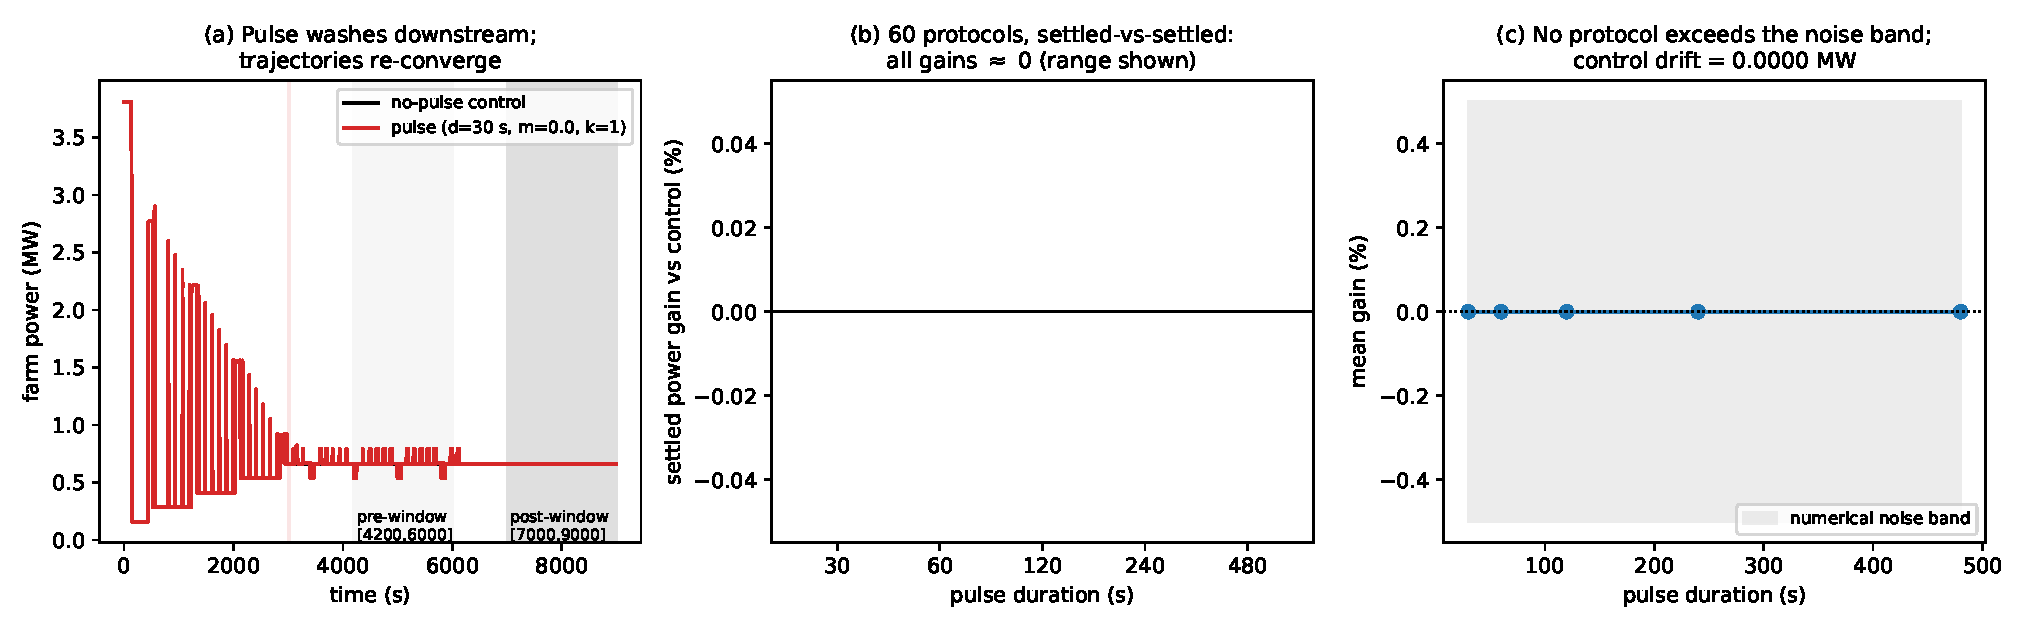
\includegraphics[width=0.98\textwidth]{figs/fig4_defib_null.pdf}
\caption{The null result. Left: control (black) and the argmax protocol (red) trajectories
re-converge after the pulse (shaded). Middle: all 60 settled-vs-settled gains. Right: no
protocol leaves the numerical-noise band; control drift $0.0000$\,MW.}
\label{fig:defib}
\end{figure}

\section{Results}

All 60 protocols: settled gains in $[-0.03\%,+0.05\%]$ (Fig.~\ref{fig:defib} middle). No
trend with duration, strength, or block size; the argmax protocol ($d=30$\,s, $m=0$,
$k=1$, $+0.05\%$) is inside the noise band. The pre-window power of pulsed runs is already
$0.3$--$0.5\%$ off the control (re-settlement still in progress inside $[4200,6000]$\,s for
the longest pulses), confirming the transient washes through rather than persisting.

\section{Where the illusion comes from}

Relax the protocol one step at a time and watch the phantom gain appear:

\begin{center}\small
\begin{tabular}{lccc}
\toprule
comparison & $T$ & ``gain'' & status\\
\midrule
settled vs settled, control-checked & 9000 s & $0.0\%$ & true effect\\
settled vs mid-settlement & 6000 s & $+5$--$+13\%$ & artifact\\
mid-settlement vs mid-settlement, $T=2000$ s & 2000 s & up to $+20\%$ & artifact\\
\bottomrule
\end{tabular}
\end{center}

The mid-settlement window sits on the relaxation transient, whose amplitude is largest at
the row tail, i.e.\ exactly where a pulse acts. The artifact magnitude decays on the
$(N-k)L/U$ scale: by $T=9000$\,s it is gone. This is a special case of the settlement law
measured in the companion paper (settle time $= (N-1)L/U$, 2--4\% error), and it quantifies
the practical bias: an A/B evaluation of any near cut-in control that ends before the row
re-settles overstates the gain. A 1600\,s evaluation at $\lambda=10$ reads $+13\%$ high
(companion paper, Fig.~5a).

\section{Mechanism}

The coupling in the model is strictly feed-forward: machine $j$ affects only $i>j$, with a
positive delay. The steady state of such a chain at fixed $(U_0,\lambda)$ is unique and is
reached by washout of any upstream transient. Two consequences: (i) a transient pulse cannot
select a different settled branch (there is no second branch to select); (ii) the pulse
changes only the power \emph{during} $[3000, 3000+d+(N-k)L/U]$, an energy that is of order
the pulse cost itself. Multistability would require a feedback loop (two-dimensional
wrapping, atmospheric recirculation into the row, or control), none of which is present in a
straight row in steady wind.

\section{What \emph{does} change the settled state}

The experiments in the companion paper identify the levers that do: (i) sustained actuation
(wake steering~\cite{Howland2019}, sustained throttle); (ii) layout (the power staircase of
the companion paper means small spacing changes near a step boundary are worth
disproportionately much in the near cut-in band); (iii) operating point (raising $U_0$ above
the band). The negative result here is the boundary condition for all three: it tells the
control community which cost class a near cut-in strategy belongs to.

\section{Limitations}

The null result is model-structural, so it should hold for any feed-forward wake model, but
we verified it in the Jensen kernel; the Gaussian kernel was checked for the argmax protocol
(same null). Two-dimensional rows, wake meander that re-captures upstream machines, and
control-induced feedback are outside the structural argument and remain open.

\section*{References}
\begin{thebibliography}{9}
\bibitem{Howland2019} Howland, M.F., Lele, S.K. \& Dabiri, J.O. 2019 \emph{Proc.\ Natl\ Acad.\ Sci.\ USA} 116(29), 14495--14500. \doi{10.1073/pnas.1903680116}.
\bibitem{Korb2020} Korb, M. \emph{et al.} 2020 \emph{Wind Energy} 23(5), 1075--1090. \doi{10.1002/we.2513}.
\bibitem{VanVondelen2024} van Vondelen, M. \emph{et al.} 2024 \emph{Wind Energy} 27, e2896. \doi{10.1002/we.2896}.
\end{thebibliography}
\end{document}
